\documentclass{beamer}

\mode<presentation> {
\usetheme{Madrid}
}

\usepackage{natbib}
\usepackage[T1]{fontenc}
\usepackage[french]{babel}
\usepackage[autolanguage]{numprint}
\usepackage{graphicx} 
\usepackage{booktabs}
\bibliographystyle{unsrtnat}
\usepackage{tabularx} 
\usepackage{amsmath}  
\usepackage{tabto}
\usepackage{amsfonts}
\usepackage{multirow}
\usepackage{caption}
\usepackage{subcaption}
\usepackage{dsfont}
\usepackage{graphicx}
\usepackage[ruled,vlined]{algorithm2e}
\usepackage{float}
\include{pythonlisting}

%----------------------------------------------------------------------------------------

\title[Complétion de données]{Transport optimal pour la complétion de données manquantes dans des séries temporelles } 

\author{Léo LAFFEACH} 
\institute[ENS Rennes] 
{
ENS Rennes\\ 
}
\date{\today} 

\begin{document}

\begin{frame}
\titlepage 
\end{frame}

\begin{frame}
\frametitle{Sommaire} 
\tableofcontents
\end{frame}


\section{Introduction}

\begin{frame}
\frametitle{Introduction}

\begin{figure}[H]
    \centering
    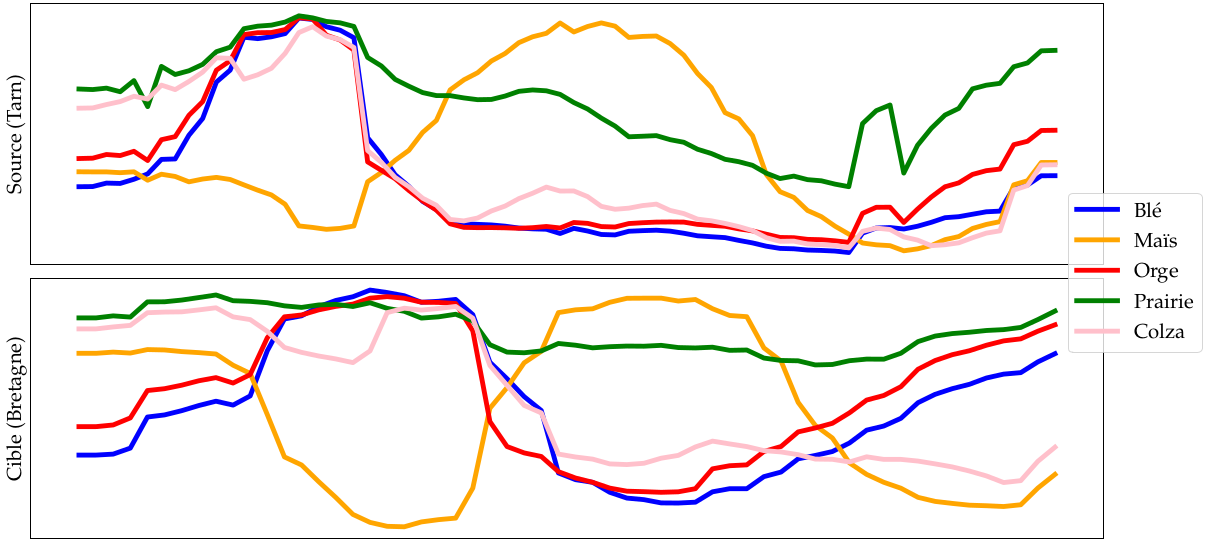
\includegraphics[scale = 0.25]{images/exemple_serie_temps.png}
    \caption{Moyennes par classe d'occupation du sol d'un indicateur de croissance de végétation pour deux zones géographiques différentes.}
    \label{exemple_intro}
\end{figure}

\end{frame}

%------------------------------------------------
\section{Transport Optimal et imputation de données manquantes}
%------------------------------------------------

\subsection{Transport Optimal} 

\begin{frame}
    \frametitle{Transport Optimal}
    Soit \textbf{X} et \textbf{X}', deux ensembles d'échantillons avec des poids, dans $\mathbb{R}^{d}$:
    $\{ (x_i, w_i) \}^{n}_{i = 1}$ avec $\sum_i w_i = 1$ et $\{ (x'_j, w'_j) \}^{n'}_{j = 1}$ avec $\sum_j w'_j = 1$.
    \begin{block}{Transport Optimal}
        $$\textbf{OT}(\textbf{X}, \textbf{X}') = \underset{\gamma \in \Gamma(\textbf{w}, \textbf{w}')}{\operatorname{\arg \min}} \langle \textbf{C}(\textbf{X}, \textbf{X}'), \gamma \rangle$$
    \end{block}
    \begin{itemize}
        \item $\Gamma(\textbf{w}, \textbf{w}') = \{ \mathbf{\gamma} | \mathbf{\gamma} \geq 0, \mathbf{\gamma} \mathds{1}_{n'} = \textbf{w}, \mathbf{\gamma}^{\top} \mathds{1}_{n} = \textbf{w}'\}$\\
        est l'ensemble de transports linéaires contraints, de telle sorte que toute la masse de \textbf{X} est transportée vers toute la masse de \textbf{X}'.
        \item $\textbf{C}(\textbf{X}, \textbf{X}') = \{d(\textbf{X}_{ij}, \textbf{X}'_{i'j'})\}$\\
        Avec $d(\textbf{X}_{ij}, \textbf{X}'_{i'j'})$ est la distance entre deux éléments de \textbf{X} et \textbf{X}'.
    \end{itemize}
\end{frame}

%------------------------------------------------

\subsection{OT avec régularisation}

\begin{frame}{Transport Optimal avec régularisation}
    Pour rendre le problème précédent différentiable, on peut ajouter une régularisation.
    \begin{block}{Transport Optimal avec régularisation}
        $$\mathbf{OT_{\epsilon}(\textbf{X}, \textbf{X}') = \underset{\gamma \in \Gamma(\textbf{w}, \textbf{w}')}{\operatorname{\arg \min}} \langle \textbf{C}(\textbf{X}, \textbf{X}'), \gamma \rangle + \epsilon \textit{h}(\gamma)}$$
    \end{block}
    \begin{itemize}
        \item $\epsilon > 0$.
        \item $\textit{h}(\gamma) = \sum_{ij}\gamma_{ij} \log \gamma_{ij}$ est l'entropie négative.
    \end{itemize}
    Cependant, dû au terme de l'entropie, $\textbf{OT}_{\epsilon}$ n'est plus forcément positif. 
\end{frame}

%----------------------

\begin{frame}{OT avec régularisation}
    Ce qui peut se résoudre via un débiaisement, en soustrayant les termes d'auto-correction.
    \begin{block}{Divergence de Sinkhorn}
        $$S_{\epsilon}(\textbf{X}, \textbf{X}') = \textbf{OT}_{\epsilon}(\textbf{X},\textbf{X}') - \frac{1}{2}(\textbf{OT}_{\epsilon}(\textbf{X}, \textbf{X}) + \textbf{OT}_{\epsilon}(\textbf{X}', \textbf{X}'))$$
    \end{block}
    Ainsi on a une équation qui est positive, convexe, et qui peut être calculée avec un faible coût additionel comparé à $\textbf{OT}_{\epsilon}$
\end{frame}

%------------------------------------------------

\subsection{Complétion de données en utilisant le transport optimal}

\begin{frame}{Complétion de données en utilisant le transport optimal}
    Soit $\Omega = (\omega_{ij})_{ij} \in \{0,1\}^{n\times d}$ un masque binaire qui indique si la donnée est observée ou non, ie: $\omega_{ij} = 1$ (resp. 0) si et seulement si l'entrée (i,j) est observée (resp. manquante). 
    \begin{block}{Valeurs observées}
        $$\textbf{X}=\textbf{X}^{(\textit{obs})}\odot \Omega + \textbf{NA} \odot (\mathbf{\mathds{1}} - \Omega)$$
    \end{block}
    \begin{itemize}
        \item $\mathbf{\textbf{X}^{(\textit{obs})}\in \mathbb{R}^{n\times d}}$ contient les données observées
        \item $\mathbf{\odot}$ est le produit élément par élément
    \end{itemize}
    \begin{block}{Valeurs imputées}
        $$\hat{\textbf{X}}=\textbf{X}^{(\textit{obs})}\odot \Omega + \hat{\textbf{X}}^{(\textit{imp})}\odot (\mathbf{\mathds{1}} - \Omega)$$
    \end{block}
    où $\hat{\textbf{X}} \in \mathbb{R}^{n\times d}$ contient les valeurs imputées.
\end{frame}

%----------------------

\begin{frame}{Complétion de données en utilisant le transport optimal}
    \begin{center}
        \scalebox{0.75}{
            \begin{minipage}{1\linewidth}
                \begin{algorithm}[H]
                    \KwIn{$\textbf{X}\in (\mathbb{R} \cup \{NA\})^{n\times d}, \Omega \in \{0,1\}^{n\times d}, \alpha, \eta, \epsilon > 0, n \geq m > 0,$}
                    \tabto{0.2cm}\textbf{Initialisation}: pour j = 1, ..., d,
                    \begin{itemize}
                        \item pour i t.q. $\omega_{ij} = 0, \hat{x}_{ij} \leftarrow \bar{x_{:j}^{\textit{obs}}} + \epsilon_{ij}\: avec\: \epsilon \sim \mathcal{N}(0,\eta)\: et\: \bar{x_{:j}^{\textit{obs}}}$ correspondant à la moyenne des données observées dans la j-ème variable (données manquantes)
                        \item pour i t.q. $\omega_{ij} = 1, \hat{x}_{ij} \leftarrow x_{ij}$ (entrées observés)
                    \end{itemize}
                    \tabto{0.2cm}$\textbf{Pour\: iter} = 1,2, ..., iter_{max}\: \textbf{faire}$
                    \tabto{1cm}Echantilloner deux ensembles $\textit{K}$ et $\textit{L}$ de $\textit{m}$ indices 
                    \tabto{1cm}$\mathcal{L}(\hat{\textbf{X}}_{\textit{K}},\hat{\textbf{X}}_{\textit{L}}) \leftarrow S_{\epsilon}(\hat{\textbf{X}}_{\textit{K}},\hat{\textbf{X}}_{\textit{L}})$
                    \tabto{1cm}$\hat{\textbf{X}}_{\textit{K} \cup \textit{L}}^{(\textit{imp})} \leftarrow \hat{\textbf{X}}_{\textit{K} \cup \textit{L}}^{(\textit{imp})} - \alpha \textbf{RMSprop}(\nabla_{\hat{\textbf{X}}_{\textit{K} \cup \textit{L}}^{(\textit{imp})}} \mathcal{L})$
                    
                    \tabto{0.2cm}$\textbf{Fin\: Pour}$
                    
                    \KwOut{$\hat{\textbf{X}}$}
                    \caption{Imputation avec Sinkhorn par lots} 
                \label{Algorithm1}
                \end{algorithm}
            \end{minipage}%
        }
    \end{center}
\end{frame}

%------------------------------------------------
\section{Match-And-Deform (MAD)}
%------------------------------------------------

\subsection{Alignement temporel dynamique}

\begin{frame}{Alignement temporel dynamique}
    $x$ et $x'$ $\in \mathbb{R}^{t\times d}$.
    \begin{block}{Dynamic Time Warping}
        $$\textbf{DTW}(x,x') = \underset{\pi \in \mathcal{A}(T, T')}{\operatorname{\arg \min}} \langle \textbf{C}(x, x'), \pi \rangle$$
    \end{block}
    \begin{itemize}
        \item $\textbf{C}(x, x') = \{d(x_{jk}, x'_{j'k'})\}$, où $d(x_{jk}, x'_{j'k'})$ est la distance entre deux éléments de $x$ et $x'$.
        \item $\mathcal{A}(T, T')$ est l'ensemble des alignements admissibles entre $x$ et $x'$. 
    \end{itemize}
    Un alignement admissible $\pi \in \mathcal{A}(T, T')$ est une matrice binaire telle que $\pi_{1,1} = \pi_{T, T'} = 1$,
    et pour chaque couple d'horodatage $(l;m)$ tel que $\pi_{l, m} = 1$, il y a soit
    $\pi_{l-1, m} = 1$ ou $\pi_{l, m-1} = 1$ ou $\pi_{l-1, m-1} = 1$.
    Les autres valeurs de $\pi$ valent 0.
\end{frame}

%------------------------------------------------

\subsection{Match-And-Deform}

\begin{frame}{Match-And-Deform}
    \begin{block}{MAD}
        \begin{equation*}
            \begin{split}
                MAD(\textbf{X}, \textbf{X}') & = \underset{\underset{\pi \in \mathcal{A}(T, T')}{\gamma \in \Gamma(w, w')}}{\operatorname{\arg \min}} \langle \textbf{L(X, X')} \otimes \mathbf{\pi, \gamma} \rangle \\
                & = \underset{\underset{\pi \in \mathcal{A}(T, T')}{\gamma \in \Gamma(w, w')}}{\operatorname{\arg \min}} \sum_{i,j} \sum_{l,m} d(x^i_l, x'^j_m) \pi_{lm} \gamma_{ij}
            \end{split}
        \end{equation*}
    \end{block}
    \begin{itemize}
        \item $\otimes$ est la multiplication tenseur-matrice
        \item $\gamma$ est le plan de transport entre les échantillons
        \item $\pi$ est le chemin DTW global qui aligne les horodatages entre \textbf{X} et \textbf{X}'.
        \item \textbf{L}(\textbf{X}, \textbf{X}') est un tenseur en 4 dimensions dont les éléments sont $\textbf{\textit{L}}^{i,j}_{l,m} = d(x^i_l, x'^j_m)$, 
              avec $d\: :\: \mathds{R}^d \times \mathds{R}^d \rightarrow \mathds{R}^+$ une distance.
    \end{itemize}
\end{frame}

%------------------------------------------------

\subsection{MAD pour l'imputation de données dans des séries temporelles}

\begin{frame}{MAD pour l'imputation de données dans des séries temporelles}
    \begin{center}
        \scalebox{0.75}{
            \begin{minipage}{1\linewidth}
                \begin{algorithm}[H]
                    \KwIn{$\textbf{X}\in (\mathbb{R} \cup \{NA\})^{n\times t\times d}, \mathbf{\Omega} \in \{0,1\}^{n\times t\times d}, \textbf{X}'\in (\mathbb{R} \cup \{NA\})^{n'\times t'\times d}, \mathbf{\Omega}' \in \{0,1\}^{n'\times t'\times d}, \alpha, \eta, \epsilon > 0, n \geq m > 0,$}
                    \tabto{0.2cm}\textbf{Initialisation}: for k = 1, ..., d,
                    \begin{itemize}
                        \item pour i pour j t.q. $\omega_{ijk} = 0, \hat{x}_{ijk} \leftarrow \bar{x_{::k}^{\textit{obs}}} + \epsilon_{ijk}\: avec\: \epsilon \sim \mathcal{N}(0,\eta)\: et\: \bar{x_{::k}^{\textit{obs}}}$ correspondant à la moyenne des données observées dans la k-ème variable (données manquantes)
                        \item pour i pour j t.q. $\omega_{ijk} = 1, \hat{x}_{ijk} \leftarrow x_{ijk}$ (données observées)
                    \end{itemize}
                    \tabto{0.2cm} faire la même chose pour la donnée cible. 
                    \tabto{0.2cm}$\textbf{Pour\: iter} = 1,2, ..., iter_{max}\: \textbf{faire}$
                    \tabto{1cm}Echantilloner deux ensembles $\textit{K}$ et $\textit{L}$ de $\textit{m}$ indices 
                    \tabto{1cm}$\mathcal{L}(\hat{\textbf{X}}_{\textit{K}},\hat{\textbf{X}}'_{\textit{L}}) \leftarrow \textbf{MAD}(\hat{\textbf{X}}_{\textit{K}},\hat{\textbf{X}}'_{\textit{L}})$
                    
                    \tabto{1cm}$\hat{\textbf{X}}_{\textit{K}}^{(\textit{imp})} \leftarrow \hat{\textbf{X}}_{\textit{K}}^{(\textit{imp})} - \alpha \textbf{RMSprop}(\nabla_{\hat{\textbf{X}}_{\textit{K}}^{(\textit{imp})}} \mathcal{L})$
                    \tabto{1cm}$\hat{\textbf{X}'}_{\textit{L}}^{(\textit{imp})} \leftarrow \hat{\textbf{X}'}_{\textit{L}}^{(\textit{imp})} - \alpha \textbf{RMSprop}(\nabla_{\hat{\textbf{X}'}_{\textit{L}}^{(\textit{imp})}} \mathcal{L})$
                    
                    \tabto{0.2cm}$\textbf{Fin\: Pour}$
                    
                    \KwOut{$\mathbf{\hat{X}}, \mathbf{\hat{X}}'$}
                    
                    
                    \caption{{Imputation avec MAD par lots} \label{Algorithm2}}
                    
                \end{algorithm}
            \end{minipage}%
        }
    \end{center}
\end{frame}

%----------------------

\begin{frame}{MAD pour l'imputation de données dans des séries temporelles}
    \begin{center}
        \scalebox{0.75}{
            \begin{minipage}{1\linewidth}
                \begin{algorithm}[H]
                    \KwIn{$\textbf{X}\in (\mathbb{R} \cup \{NA\})^{n\times t\times d}, \mathbf{\Omega} \in \{0,1\}^{n\times t\times d}, \textbf{X}'\in (\mathbb{R} \cup \{NA\})^{n'\times t'\times d}, \mathbf{\Omega}' \in \{0,1\}^{n'\times t'\times d}, \alpha, \eta, \epsilon > 0, n \geq m > 0,$}
                    \tabto{0.2cm}\textbf{Initialisation}: for k = 1, ..., d,
                    \begin{itemize}
                        \item pour i pour j t.q. $\omega_{ijk} = 0, \hat{x}_{ijk} \leftarrow \bar{x_{::k}^{\textit{obs}}} + \epsilon_{ijk}\: avec\: \epsilon \sim \mathcal{N}(0,\eta)\: et\: \bar{x_{::k}^{\textit{obs}}}$ correspondant à la moyenne des données observées dans la k-ème variable (données manquantes)
                        \item pour i pour j t.q. $\omega_{ijk} = 1, \hat{x}_{ijk} \leftarrow x_{ijk}$ (données observées)
                    \end{itemize}
                    \tabto{0.2cm} faire la même chose pour la donnée cible. 
                    \tabto{0.2cm}$\textbf{Pour\: iter} = 1,2, ..., iter_{max}\: \textbf{faire}$
                    \tabto{1cm}Echantilloner quatre ensembles $\textit{K}$, $\textit{L}$, $\textit{K}'$ et $\textit{L}'$ de $\textit{m}$ indices 
                    \tabto{1cm}$\mathcal{L}(\hat{\textbf{X}}_{\textit{K}},\hat{\textbf{X}}'_{\textit{L}}) \leftarrow \textbf{MAD}(\hat{\textbf{X}}_{\textit{K}},\hat{\textbf{X}}'_{\textit{L}}) + S_{\epsilon}(\hat{\textbf{X}}'_{\textit{K'}},\hat{\textbf{X}}'_{\textit{L'}})$
                    
                    \tabto{1cm}$\hat{\textbf{X}}_{\textit{K}}^{(\textit{imp})} \leftarrow \hat{\textbf{X}}_{\textit{K}}^{(\textit{imp})} - \alpha \textbf{RMSprop}(\nabla_{\hat{\textbf{X}}_{\textit{K}}^{(\textit{imp})}} \mathcal{L})$
                    \tabto{1cm}$\hat{\textbf{X}'}_{\textit{K}' \cup \textit{L} \cup \textit{L}'}^{(\textit{imp})} \leftarrow \hat{\textbf{X}'}_{\textit{K}' \cup \textit{L} \cup \textit{L}'}^{(\textit{imp})} - \alpha \textbf{RMSprop}(\nabla_{\hat{\textbf{X}'}_{\textit{K}' \cup \textit{L} \cup \textit{L}'}^{(\textit{imp})}} \mathcal{L})$
                    
                    \tabto{0.2cm}$\textbf{Fin\: Pour}$
                    
                    \KwOut{$\mathbf{\hat{X}}, \mathbf{\hat{X}}'$}
                    
                    
                    \caption{{Imputation avec MAD et Sinkhorn par lots} \label{Algorithm3}}
                    
                \end{algorithm}
            \end{minipage}%
        }
    \end{center}
\end{frame}

%------------------------------------------------
\section{Expérience}
%------------------------------------------------

\begin{frame}{Racine de l'Erreur Quadratique Moyenne}
    On considère la racine de l'erreur quadratique moyenne comme mesure pour évaluer la complétion.
    \begin{block} {Racine de l'Erreur Quadratique Moyenne}
        $$\sqrt{\frac{1}{m_0} \sum_{(i,j)|\omega_{ij} = 0} (x^{true}_{i,j} - \hat{x}_{i,j})^2 }$$
    \end{block}
\end{frame}

%------------------------------------------------

\subsection{Génération synthétique de données manquantes}

\begin{frame}{Génération synthétique de données manquantes}
    \begin{itemize}
        \item \textbf{Manquantes au hasard} :\\
            Choisir des couples $(j,k) \in \{0, 1, ..., t\}\times \{0, 1, ..., d\}$ et de les considérer comme manquant pour tout $i \in \{0, 1, ..., n\}$.

        \item \textbf{Manquantes avec un biais} :\\
            Choisir des horodatages et d'y supprimer les données pour tout $i \in \{0, 1, ..., n\}$.
    \end{itemize}
    
\end{frame}

%------------------------------------------------

\subsection{Manquantes au hasard}


\begin{frame}{Manquantes au hasard}
    \begin{center}
        \scalebox{0.5}{
            \begin{minipage}{1.2\linewidth}
                \begin{table}[H]
                    \begin{tabular}{| c | c | c | c | c | c |}
                        \hline
                        Pourcentage de & Problèmes & Moyenne & Sinkhorn & MAD & MAD + \\
                        données manquantes &  &  &  &  & Sinkhorn \\[0.5ex]
                        \hline\hline
                        \multirow{5}{4em}{50\%} & DK1 $\rightarrow$ FR1 & 1.2469 & 1.2528 & \underline{1.1015} & \textbf{1.0843} \\
                                                & DK1 $\rightarrow$ FR2 & 1.1294 & 1.1305 & \underline{1.0366} & \textbf{1.0345} \\
                                                & DK1 $\rightarrow$ AT1 & 1.1920 & 1.1944 & \textbf{1.0343} & \underline{1.0346} \\
                                                & FR1 $\rightarrow$ DK1 & 1.1862 & 1.1894 & \underline{1.0537} & \textbf{1.0501} \\
                                                & FR1 $\rightarrow$ FR2 & 1.1294 & 1.1305 & \underline{1.0540} & \textbf{1.0525} \\
                        \hline  
                        \multirow{5}{4em}{60\%} & DK1 $\rightarrow$ FR1 & 1.2575 & 1.2614 & \underline{1.1128} & \textbf{1.1061} \\
                                                & DK1 $\rightarrow$ FR2 & 1.1134 & 1.1141 & \underline{1.0407} & \textbf{1.0390} \\
                                                & DK1 $\rightarrow$ AT1 & 1.1699 & 1.1716 & \underline{1.0321} & \textbf{1.0286} \\
                                                & FR1 $\rightarrow$ DK1 & 1.1772 & 1.1791 & \textbf{1.0567} & \underline{1.0568} \\
                                                & FR1 $\rightarrow$ FR2 & 1.1134 & 1.1141 & \underline{1.0486} & \textbf{1.0480} \\
                        \hline 
                        \multirow{5}{4em}{70\%} & DK1 $\rightarrow$ FR1 & 1.2577 & 1.2599 & \underline{1.1036} & \textbf{1.1004} \\
                                                & DK1 $\rightarrow$ FR2 & 1.0620 & 1.0627 & \underline{1.0109} & \textbf{1.0055} \\
                                                & DK1 $\rightarrow$ AT1 & 1.1894 & 1.1904 & \underline{1.0645} & \textbf{1.0624} \\
                                                & FR1 $\rightarrow$ DK1 & 1.2021 & 1.2031 & \underline{1.1075} & \textbf{1.1038} \\
                                                & FR1 $\rightarrow$ FR2 & 1.0620 & 1.0627 & \underline{1.0303} & \textbf{1.0299} \\
                        \hline 
                        \multirow{5}{4em}{80\%} & DK1 $\rightarrow$ FR1 & 1.2614 & 1.2626 & \underline{1.1256} & \textbf{1.1233} \\
                                                & DK1 $\rightarrow$ FR2 & 1.1067 & 1.1072 & \underline{1.0305} & \textbf{1.0298} \\
                                                & DK1 $\rightarrow$ AT1 & 1.2003 & 1.2016 & \underline{1.0820} & \textbf{1.0806} \\
                                                & FR1 $\rightarrow$ DK1 & 1.2267 & 1.2311 & \underline{1.1165} & \textbf{1.1151} \\
                                                & FR1 $\rightarrow$ FR2 & 1.1067 & 1.1072 & \underline{1.0748} & \textbf{1.0746} \\
                        \hline
                        \multirow{5}{4em}{90\%} & DK1 $\rightarrow$ FR1 & 1.2635 & 1.2605 & \underline{1.1405} & \textbf{1.1389} \\
                                                & DK1 $\rightarrow$ FR2 & 1.0932 & 1.0937 & \underline{1.0441} & \textbf{1.0436} \\
                                                & DK1 $\rightarrow$ AT1 & 1.1977 & 1.1961 & \textbf{1.0863} & \underline{1.0900} \\
                                                & FR1 $\rightarrow$ DK1 & 1.2266 & 1.2247 & \underline{1.1252} & \textbf{1.1240} \\
                                                & FR1 $\rightarrow$ FR2 & 1.0932 & 1.0937 & \textbf{1.0549} & \underline{1.0588} \\
                        \hline 
                    \end{tabular}
                \caption{Valeurs de RMSE pour différents pourcentages de données manquantes à 1000 itérations}    
                \end{table}
            \end{minipage}%
        }
    \end{center}
\end{frame}

%------------------------------------------------

\subsection{Manquantes avec un biais}

\begin{frame}{Manquantes avec un biais}
    \begin{center}
        \scalebox{0.5}{
            \begin{minipage}{1.2\linewidth}
                \begin{table}[H]
                    \begin{tabular}{| c | c | c | c | c | c |}
                        \hline
                        Pourcentage de & Problèmes & Moyenne & Sinkhorn & MAD & MAD + \\
                        données manquantes &  &  &  &  & Sinkhorn \\[0.5ex]
                        \hline\hline
                        \multirow{5}{4em}{50\%} & DK1 $\rightarrow$ FR1 & 1.1238 & 1.1313 & \textbf{1.0579} & \underline{1.0604} \\
                                                & DK1 $\rightarrow$ FR2 & 1.0147 & 1.0167 & \textbf{0.9488} & \underline{0.9510} \\
                                                & DK1 $\rightarrow$ AT1 & 0.9867 & 0.9911 & \underline{0.9273} & \textbf{0.9248} \\
                                                & FR1 $\rightarrow$ DK1 & 1.1694 & 1.1725 & \underline{1.1412} & \textbf{1.1390} \\
                                                & FR1 $\rightarrow$ FR2 & 1.0147 & 1.0167 & \underline{0.9885} & \textbf{0.9477} \\
                        \hline  
                        \multirow{5}{4em}{60\%} & DK1 $\rightarrow$ FR1 & 1.2083 & 1.2144 & \underline{1.1503} & \textbf{1.1139} \\
                                                & DK1 $\rightarrow$ FR2 & 1.0465 & 1.0478 & \underline{0.9877} & \textbf{0.9853} \\
                                                & DK1 $\rightarrow$ AT1 & 0.9534 & 0.9574 & \textbf{0.9424} & \underline{0.9445} \\
                                                & FR1 $\rightarrow$ DK1 & \textbf{1.1259} & \underline{1.1286} & 1.1374 & 1.1390 \\
                                                & FR1 $\rightarrow$ FR2 & \textbf{1.0465} & \underline{1.0478} & 1.1040 & 1.1013 \\
                        \hline 
                        \multirow{5}{4em}{70\%} & DK1 $\rightarrow$ FR1 & 1.2415 & 1.2454 & \underline{1.1111} & \textbf{1.1087} \\
                                                & DK1 $\rightarrow$ FR2 & 0.9793 & 0.9810 & \underline{0.9772} & \textbf{0.9767} \\
                                                & DK1 $\rightarrow$ AT1 & 0.9734 & 0.9757 & \underline{0.9538} & \textbf{0.9536} \\
                                                & FR1 $\rightarrow$ DK1 & 1.2088 & 1.2104 & \textbf{1.1429} & \underline{1.1505} \\
                                                & FR1 $\rightarrow$ FR2 & \textbf{0.9793} & \underline{0.9810} & 0.9902 & 1.0016 \\
                        \hline 
                        \multirow{5}{4em}{80\%} & DK1 $\rightarrow$ FR1 & 1.2400 & 1.2429 & \underline{1.1791} & \textbf{1.1710} \\
                                                & DK1 $\rightarrow$ FR2 & 1.0273 & 1.0283 & \underline{1.0234} & \textbf{1.0223} \\
                                                & DK1 $\rightarrow$ AT1 & 1.0578 & 1.0587 & \underline{0.9984} & \textbf{0.9978} \\
                                                & FR1 $\rightarrow$ DK1 & 1.2590 & 1.2599 & \underline{1.2187} & \textbf{1.2180} \\
                                                & FR1 $\rightarrow$ FR2 & 1.0273 & 1.0283 & \textbf{1.0122} & \underline{1.0140} \\
                        \hline
                        \multirow{5}{4em}{90\%} & DK1 $\rightarrow$ FR1 & 1.2329 & 1.2352 & \underline{1.1453} & \textbf{1.1442} \\
                                                & DK1 $\rightarrow$ FR2 & \textbf{1.0631} & \underline{1.0639} & 1.1570 & 1.1580 \\
                                                & DK1 $\rightarrow$ AT1 & \textbf{1.0473} & \underline{1.0484} & 1.0538 & 1.0542 \\
                                                & FR1 $\rightarrow$ DK1 & 1.2394 & 1.2402 & \textbf{1.1556} & \underline{1.1626} \\
                                                & FR1 $\rightarrow$ FR2 & \textbf{1.0631} & \underline{1.0639} & 1.1294 & 1.1296 \\
                        \hline 
                    \end{tabular}
                \caption{Valeurs de RMSE pour différents pourcentages de données manquantes à 1000 itérations}    
                \end{table}
            \end{minipage}%
        }
    \end{center}
\end{frame}

%------------------------------------------------

\subsection{Evolution de la RMSE en fonction du nombre d'itérations}

\begin{frame}{Evolution de la RMSE en fonction du nombre d'itérations}
    \begin{center}
        \scalebox{0.8}{
            \begin{minipage}{1.2\linewidth}
                \begin{figure}[H]
                    \begin{subfigure}[b]{0.4\textwidth}
                        \centering
                        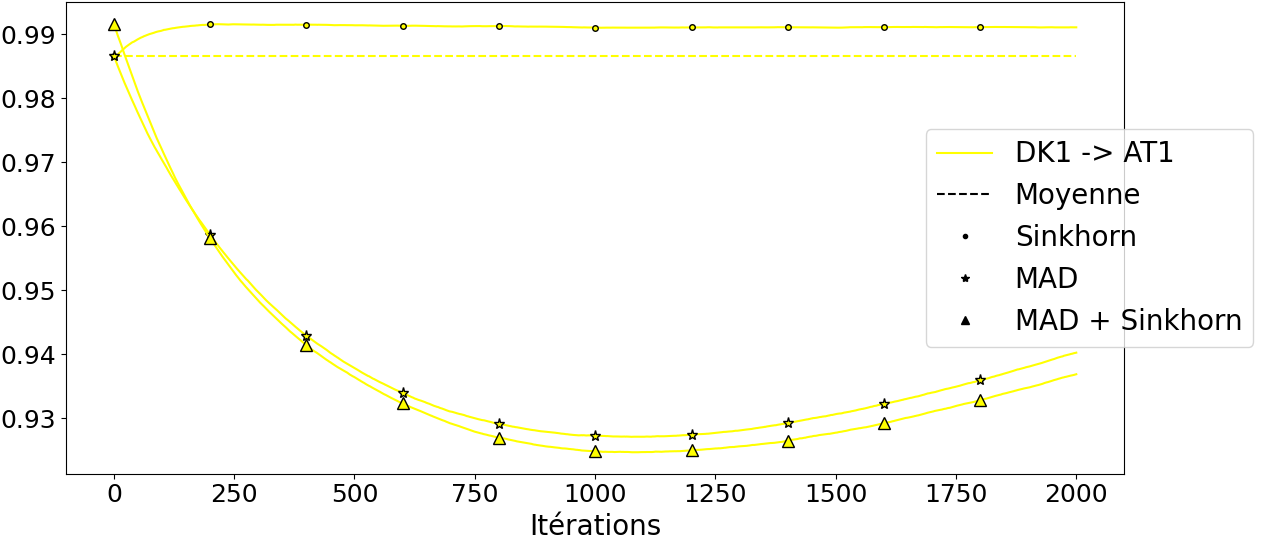
\includegraphics[scale=0.14]{images/50_biais_AT1.png}
                        \caption{50\% de données manquantes}
                        \label{50_biais_AT1}
                    \end{subfigure}
                    \hfill
                    \begin{subfigure}[b]{0.4\textwidth}
                        \raggedleft
                        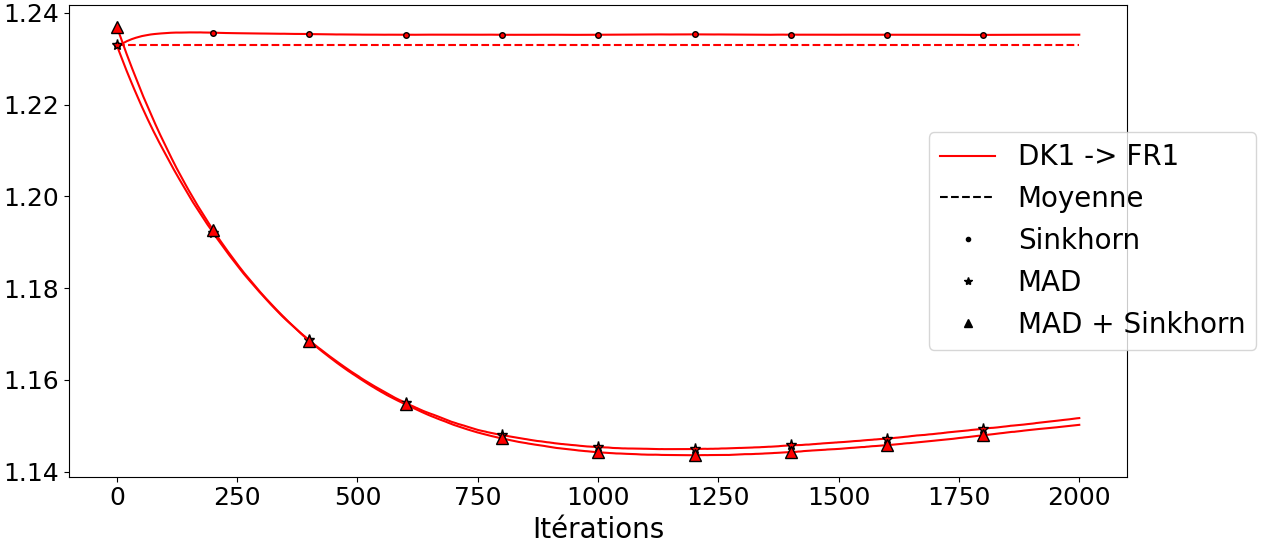
\includegraphics[scale=0.14]{images/90_biais_FR1.png}
                        \caption{90\% de données manquantes}
                        \label{90_biais_FR1}
                    \end{subfigure}
                    \caption{RMSE en fonction du nombre d'itérations}
                \end{figure}
            \end{minipage}%
        }
    \end{center}
\end{frame}


%----------

\begin{frame}{Evolution de la RMSE en fonction du nombre d'itérations}
    \begin{center}
        \scalebox{0.8}{
            \begin{minipage}{1.2\linewidth}
                \begin{figure}[H]
                    \centering
                    \begin{subfigure}[b]{0.4\textwidth}
                        \centering
                        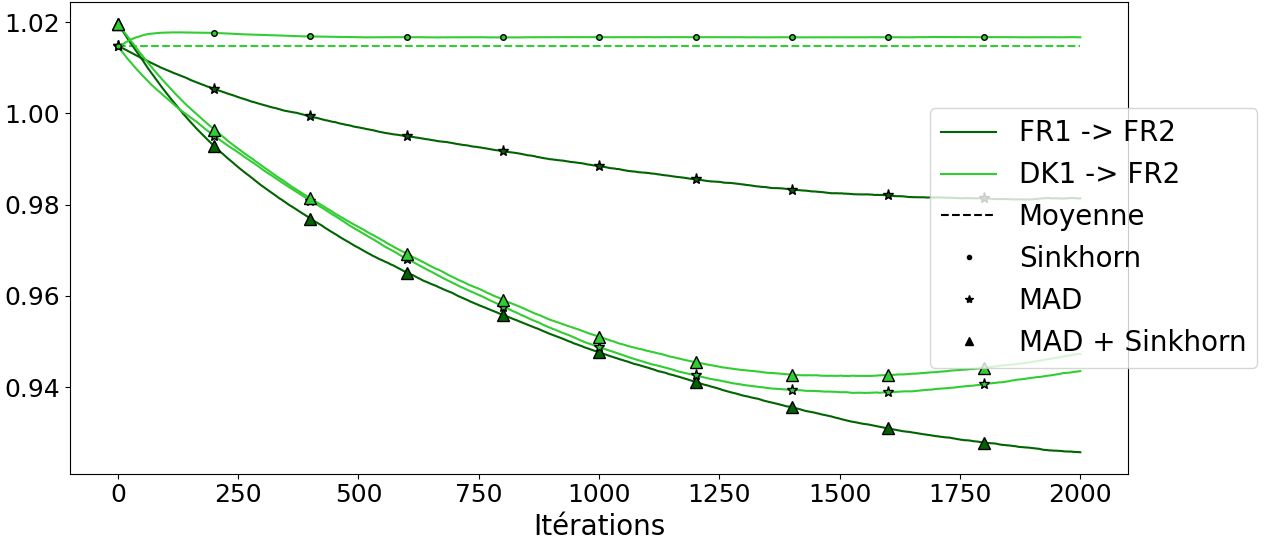
\includegraphics[scale=0.14]{images/50_biais_FR2.png}
                        \caption{50\% de données manquantes}
                        \label{50_biais_FR2}
                    \end{subfigure}
                    \hfill
                    \begin{subfigure}[b]{0.4\textwidth}
                        \centering
                        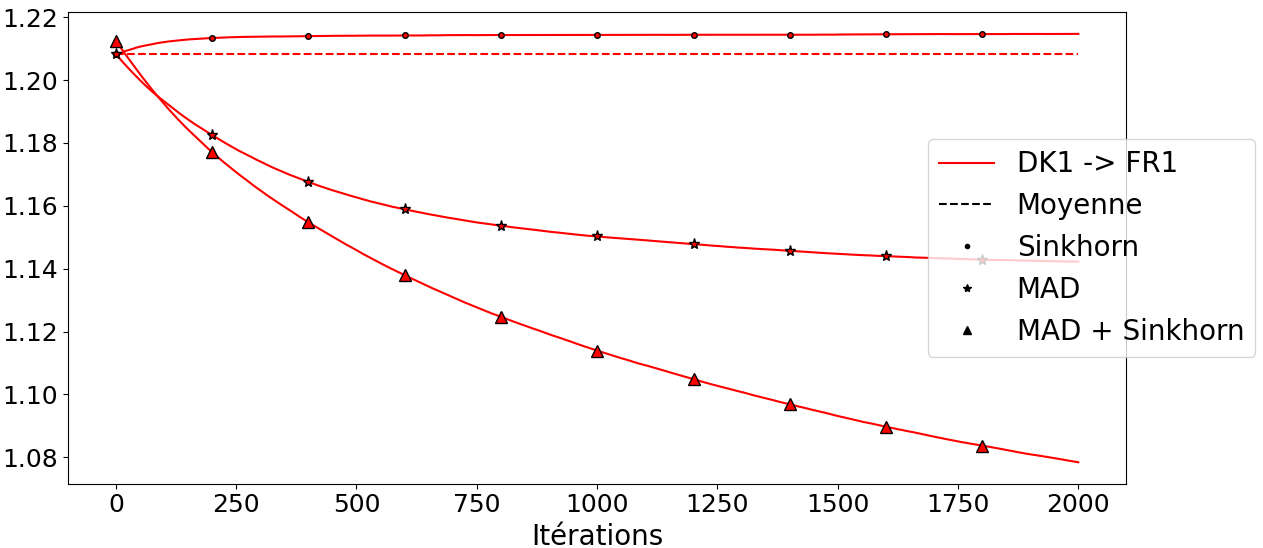
\includegraphics[scale=0.14]{images/60_biais_FR1.png}
                        \caption{60\% de données manquantes}
                        \label{60_biais_FR1}
                    \end{subfigure}
                    \hfill
                    \begin{subfigure}[b]{0.4\textwidth}
                        \centering
                        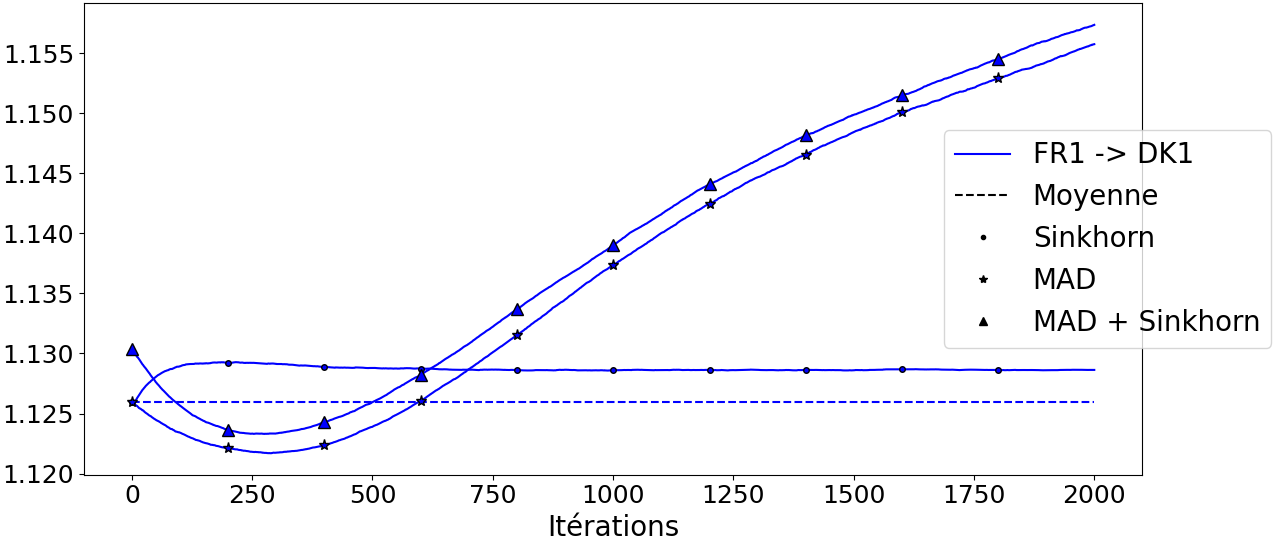
\includegraphics[scale=0.14]{images/60_biais_DK1.png}
                        \caption{60\% de données manquantes}
                        \label{60_biais_DK1}
                    \end{subfigure}
                    \hfill
                    \begin{subfigure}[b]{0.4\textwidth}
                        \centering
                        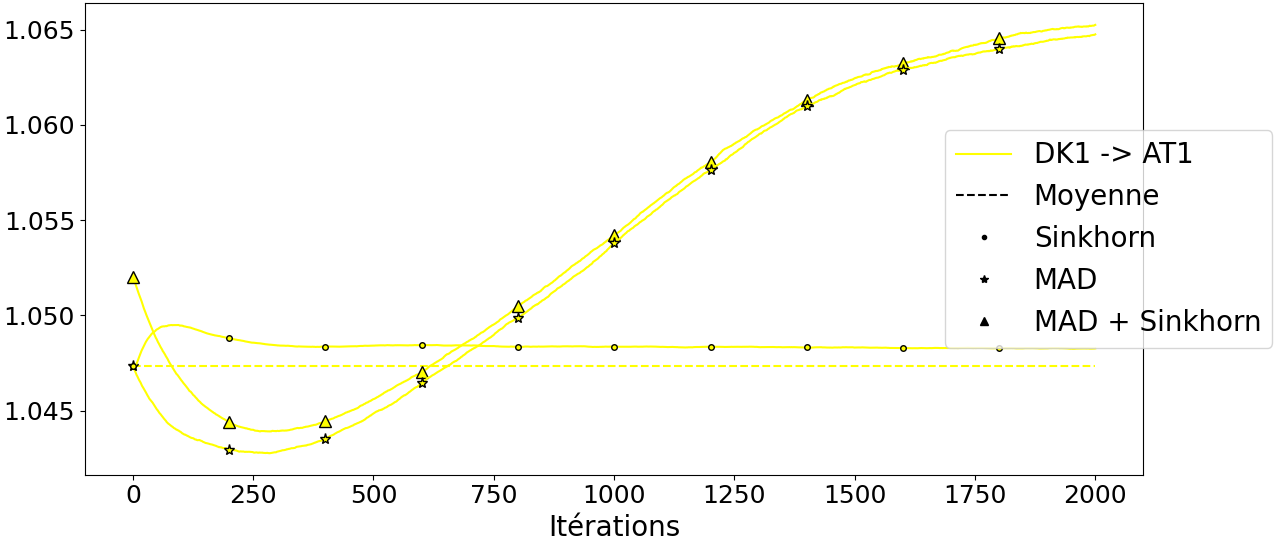
\includegraphics[scale=0.14]{images/90_biais_AT1.png}
                        \caption{90\% de données manquantes}
                        \label{90_biais_AT1}
                    \end{subfigure}
                    \caption{RMSE en fonction du nombre d'itérations}
                \end{figure}
            \end{minipage}%
        }
    \end{center}
\end{frame}

%------------------------------------------------
\section{Conclusion}
%------------------------------------------------
\begin{frame}{Conclusion}
    \Huge{\centerline{Conclusion}}
\end{frame}

%------------------------------------------------

\end{document}